\documentclass{../zirkelblatt1415}
\setlength\parskip{\medskipamount}
\setlength\parindent{0pt}
\pagestyle{empty}

\usepackage{geometry}
\geometry{top=2cm,bottom=2cm}

\begin{document}
\sffamily

\newcommand{\zettel}{
  \Huge Folgende Augenzahlen kamen schon:

  \begin{center}
  \begin{tabular}{cccccc}
    \scalebox{2}{\Huge$\square$} &
    \scalebox{2}{\Huge$\square$} &
    \scalebox{2}{\Huge$\square$} &
    \scalebox{2}{\Huge$\square$} &
    \scalebox{2}{\Huge$\square$} &
    \scalebox{2}{\Huge$\square$} \\
    1 & 2 & 3 & 4 & 5 & 6
  \end{tabular}
  \end{center}

  \marginpar{\vspace*{-10em}\hspace*{-2em}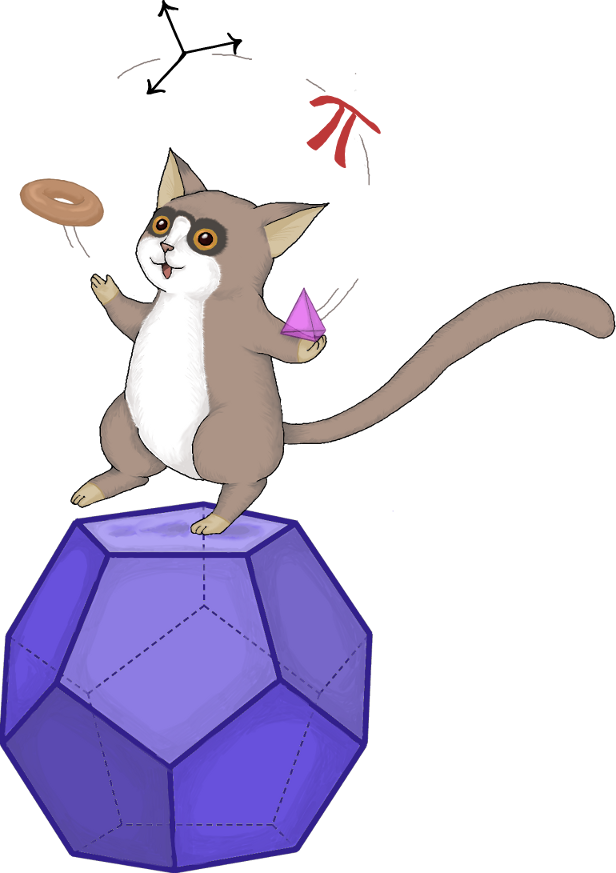
\includegraphics[scale=0.1]{images/gregor}}

  Insgesamt habe ich so oft gewürfelt (Strichliste führen):

  \hrulefill

  \normalsize Simulation im Browser: \url{http://tiny.cc/zufall}
}

\zettel\vfill
\zettel\vfill
\zettel

\end{document}
